%!tex program = lualatex
\documentclass[answers]{exam}
\usepackage{ctex}
\usepackage{graphicx}
\usepackage[margin=2cm]{geometry}
\usepackage{amsmath}
\usepackage{csquotes}
\usepackage{amssymb}
\usepackage{tikz}
\usetikzlibrary{
angles,
backgrounds,
calc,
decorations.pathmorphing,
decorations.pathreplacing,
decorations.text,
intersections,
patterns,
quotes,
shapes,
shapes.symbols,
}
\pagestyle{empty}
\newcounter{xcord}
\newcounter{ycord}
\newcounter{total}
% \ctexset{
% 	subsection/name = {第,题},
% 	subsection/number = {\thesubsection},
% 	section ={
% 		name = {第,部分}
% 	}
% }
\renewcommand{\labelenumi}{\textbf{\ifnum\value{enumi}<10 0\fi\arabic{enumi})}}

\CorrectChoiceEmphasis{\color{blue!70!green}\bfseries}

\includeonly{svsu2022level1}
\begin{document}
%!tex program = lualatex
\documentclass{exam}
\usepackage{ctex}
\usepackage{graphicx}
\usepackage[margin=2cm]{geometry}
\usepackage{amsmath, amssymb}
\usepackage{csquotes}
\usepackage{tikz, pgfplots}
\usetikzlibrary{
	angles,
	backgrounds,
	calc,
	decorations.pathmorphing,
	decorations.pathreplacing,
	decorations.text,
	intersections,
	patterns,
	quotes,
	shapes,
	shapes.symbols,
}
\pagestyle{empty}
\newcounter{xcord}
\newcounter{ycord}
\newcounter{total}
\renewcommand{\labelenumi}{\textbf{\ifnum\value{enumi}<10 0\fi\arabic{enumi})}}

\pgfplotsset{compat=1.18}

\CorrectChoiceEmphasis{\color{blue!70!green}\bfseries}
\renewcommand{\solutiontitle}{\textbf{解:}}

\usepackage{array, tabularx}
\newcolumntype{C}{>{\centering\arraybackslash}X}
\newcolumntype{B}{>{\centering\bfseries\arraybackslash}X}
\catcode`\幺=0

\begin{document}
\section{求阴影面积}
\begin{figure}[htbp]
	\centering
	\begin{gather*}
		长方形ABCD\\
		AB = 9 \\
		BC = 6 \\
		求阴影面积
	\end{gather*}
	\begin{tikzpicture}[scale=.5]
		\coordinate (A) at (9,0);
		\coordinate (B) at (0,0);
		\coordinate (C) at (0,-6);
		\coordinate (D) at (9, -6);
		\coordinate (E) at (3, 0);
		\coordinate (F) at (5, -6);
		\coordinate (C') at (9, -3);
		\coordinate (B') at ($(C') ! 1.2 ! -90:(F)$);
		\path [name path=B'C'] (B') -- (C');
		\path [name path=AE] (A) -- (E);

		\draw [name intersections={of=B'C' and AE, by=G}];
		\node [above right] at(G){$G$};

		% \path[draw=red] {AE};

		\draw[dashed](B) -- (E);
		\draw (E)-- (A) -- (D) -- (F) -- (E);
		\draw[dashed] (F) -- (C) -- (B);
		\draw (F) -- (C') -- (B') -- (E);

		\draw [pattern=north east lines](E) -- (G) -- (C') -- (F) -- cycle;
		\node at (A)[above right]{$A$};
		\node at (B)[above left]{$B$};
		\node at (C)[below left]{$C$};
		\node at (D)[below right]{$D$};
		\node at (F)[below]{$F$};
		\node at (C')[right]{$C\prime$ 中点};
		\node at (E)[above left]{$E$};
		\node at (B')[right, xshift=5pt]{$B\prime$};
	\end{tikzpicture}
\end{figure}

\begin{align}
	FC + FD                    & = 9                      \\
	FC^2                       & = FD^2 + DC^2 = FD^2 + 9 \\
	(FC + FD) \times (FC - FD) & = 9                      \\
	FC - FD                    & = 1                      \\
	FC                         & = 5
\end{align}

Calculate the length of $BE$:
\begin{align}
	\triangle CDF            & \approx \triangle CAG                               \\
	\frac{GA}{AC}            & = \frac{CD}{FD} = \frac{3}{4}                       \\
	GA                       & = \frac{9}{4}                                       \\
	GC                       & = \sqrt{GA^2 + AC^2} = \frac{15}{4}                 \\
	BG                       & = BC - GC = 6 - \frac{15}{4}     = \frac{9}{4} = GA \\
	\because \triangle GBE   & \approx \triangle GAC                               \\
	\therefore \triangle GBE & \cong \triangle GAC                                 \\
	BE                       & = AC = 3
\end{align}

\section*{20以内两位数乘法练习}
\begin{center}
	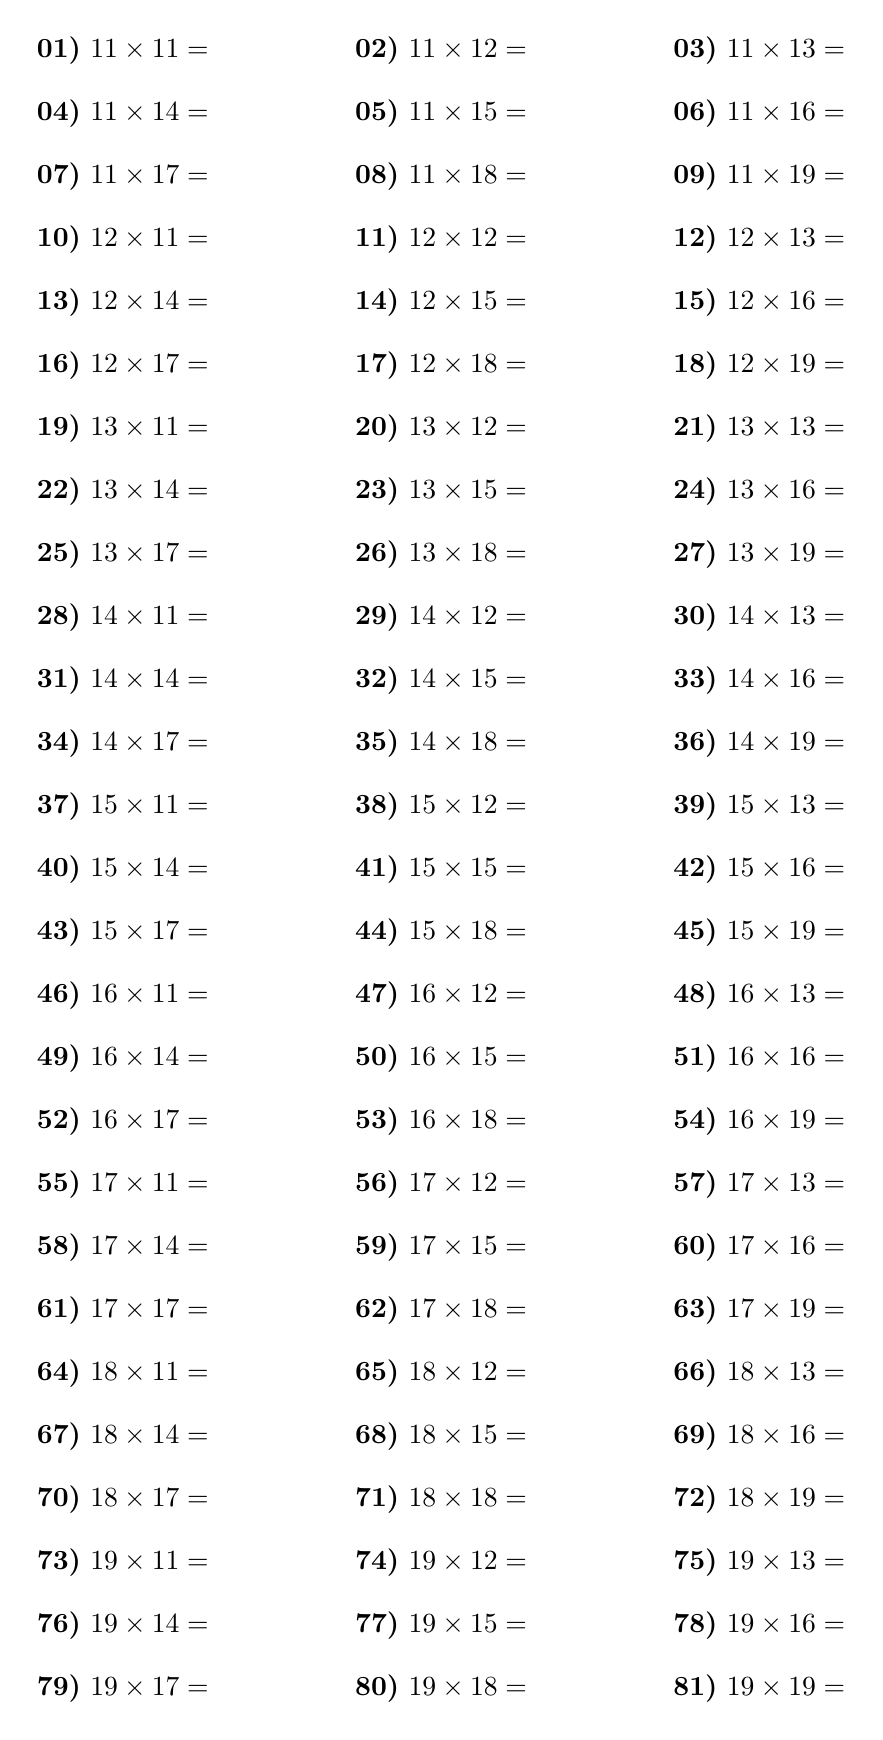
\begin{tikzpicture}
		\foreach \x in {11,...,19}
		\foreach \y in {11,...,19}
			{
				\stepcounter{total}
				\node at (\value{xcord} * \textwidth / 3, -\value{ycord}*0.8) {\textbf{\ifnum\value{total}<10
				0\fi\thetotal)} $\x \times \y =$};
		\stepcounter{xcord}		\ifnum\value{xcord}=3
		\setcounter{xcord}{0}
		\stepcounter{ycord}
		\fi
		}
	\end{tikzpicture}

\end{center}

\section{速算及巧算}
\subsection{计算总和}
\begin{enumerate}
	\item $1-2+3-4+5-6+7-8+9-10+11=$

	\item $3+5+7+9+11+13+15+17+19+21=$

	\item $100-99+98-97+96-95+94-93+93-92+91=$

	\item $6+8+10+12+14+16+18+20+22+24=$

	\item $1 + 2 + 3 + \ldots + 100 = $

	\item $2 + 4 +6 + \ldots + 100 = $

	\item $1 + 3 + 5 + \ldots + 99 = $

	\item $5 + 10 + 15 + \ldots + 100 = $

	\item $1 - (1+2) + (1+2+3) - (1+2+3+4) + \ldots - (1+2+\ldots+98) + (1+2+\ldots+99) = $

	\item $1-2+3-4+\ldots+2023-2024+2025=$

	\item $19+28+37+46+55+64+73+82+91+ \underline{\hspace{1cm}}=550$

	\item $2000-180+220-180+220-180+220-180+220-180+220=$

	\item $352.46-35.58-65.93-76.07-24.42=$

	\item $1+2+4+8+16+32+64+128+256+512+1024=$

	\item $8+89+899+8999+89999=$

	\item $8+88+888+8888+88888=$

	\item $28+208+2008+20008=$

	\item $24+63+52+17+49+81+74+38+95=$

	\item $1999.9+199.9+19.9+1.9=$

	\item $(7+9+11+13+\ldots+37)-(9+11+13+15+\ldots+35)=$

\end{enumerate}

\pagebreak
\section{速算和巧算2}

\begin{enumerate}

	\item $(6+8+10+12+\ldots+36)-(8+10+12+14+\ldots+34)=$

	\item $(1+4+7+10+\ldots+40)-(4+7+10+13+\ldots+37)=$
\end{enumerate}
\end{document}

%!tex program = lualatex
\documentclass[answers]{exam}
\usepackage{ctex}
\usepackage{graphicx}
\usepackage[margin=2cm]{geometry}
\usepackage{amsmath, amssymb}
\usepackage{csquotes}
\usepackage{tikz, pgfplots}
\usetikzlibrary{
	angles,
	backgrounds,
	calc,
	decorations.pathmorphing,
	decorations.pathreplacing,
	decorations.text,
	intersections,
	patterns,
	quotes,
	shapes,
	shapes.symbols,
}
\pagestyle{empty}
\newcounter{xcord}
\newcounter{ycord}
\newcounter{total}
\renewcommand{\labelenumi}{\textbf{\ifnum\value{enumi}<10 0\fi\arabic{enumi})}}

\pgfplotsset{compat=1.18}

\CorrectChoiceEmphasis{\color{blue!70!green}\bfseries}
\renewcommand{\solutiontitle}{\textbf{解:}}

\usepackage{array, tabularx}
\newcolumntype{C}{>{\centering\arraybackslash}X}
\newcolumntype{B}{>{\centering\bfseries\arraybackslash}X}
\catcode`\幺=0

\begin{document}

\begin{questions}
	\question 考虑方程$p(x): ax^2 + bx + c=0$,其系数$a$,$b$和$c$都是非零的,并且每个系数都满足从方程$p(x)$
	中移除包含该系数的项后得到的方程;例如,系数$b$是方程 $ax^2+c=0$的一个解。求方程$p(x)$
	所有解的和是多少?

	\begin{oneparchoices}
		\choice 总是 1 \choice 总是 -1 \choice 总是 2 \CorrectChoice 1 或者 -1 \choice 1 或者 2
	\end{oneparchoices}
	\begin{solution}
		方程$p(x)$的两个解分别为$\displaystyle x_1, x_2 = \frac{-b \pm \sqrt{b^2 - 4ac}}{2a}$,则$\displaystyle x_1 +
			x_2 = -\frac{b}{a}$\\
		由题意得
		\begin{align}
			ac^2  + bc & = 0 \label{\thequestion:1} \\
			ab^2  + c  & = 0 \label{\thequestion:2} \\
			ab    + c  & = 0 \label{\thequestion:3}
		\end{align}
		由式(\ref{\thequestion:2}) 和(\ref{\thequestion:3})得$b=1$和$a+c=0$,代入(\ref{\thequestion:1})得:
		\begin{equation}
			a(-a)^2 -a  = 0
		\end{equation}

		则$a=\pm 1$或$a=0$,因为题目中$a \ne 0$,所以$a=\pm 1$,则$\displaystyle x_1 + x_2 = -\frac{b}{a}=\pm 1$
	\end{solution}
	\question 一支行进乐队共有150名成员。有一天,只有部分成员到场,但没有人想花时间去清点具体人数。他们首先尝试以每排5名成员的方式排队,但结果多出了1名成员。接着他们改以每排6名成员的方式排列,仍然多出了1名成员。最后,他们尝试以每排7名成员的方式排列,这次多出了2名成员。请问,为了确保没有成员被剩下,他们应该以每排多少人的方式排列?

	\begin{oneparchoices}
		\choice 4人每排
		\CorrectChoice 11人每排
		\choice 13人每排
		\choice 17人每排
		\choice 上述选项中无正确答案
	\end{oneparchoices}
	\begin{solution}
		设当天一共到场$x$人, 根据题意得
		\begin{equation}
			\begin{cases}
				x \equiv 1 \pmod 5 \\
				x \equiv 1 \pmod 6
			\end{cases}
		\end{equation}
		则$x=k(5 \times 6) + 1$,其中$k=0,1,2,3 \ldots$

		根据总人数小于150这个条件,$x$可能的值有$1,31,61,91,121$,然后根据每排排7人的情况下多出2名成员,得到$x=121$,则每排11个人可以确保没有成员被剩下。

	\end{solution}

	\question 下列陈述中,哪一个是唯一正确的?
	\begin{choices}
		\choice 水平线的图形不可能有任何与x轴的交点。
		\CorrectChoice 水平线的图形不能有一个唯一的与x轴的交点,但可能有超过一个与x轴的交点。
		\choice 抛物线的图形不能有一个唯一的与x轴的交点,但可能有超过一个与x轴的交点。
		\choice 三次或更高次的多项式的图形必须至少有一个与x轴的交点。
		\choice 要么没有一个是正确的,要么不止一个正确。
	\end{choices}
	\begin{solution}\\
		选项A:当$x=0$时与$x$轴有无穷多个交点。\\
		选项B:根据以上,此描述正确。\\
		选项C:当抛物线的顶点位于$x$轴上时有唯一的交点,所以此描述错误。\\
		选项D:比如$x^4+1$这样的曲线就没有与$x$轴的交点,所以此描述错误。
	\end{solution}

	\question 下列哪个选项等于10的阶乘($10!$)。如果你对符号不熟悉,$n!$(读作\enquote{n的阶乘})对于任何非负整数$n$定义如下:
	\begin{equation*}
		\begin{cases}
			0! = 1 \\
			n > 0,n! = n \cdot (n-1)!
		\end{cases}
	\end{equation*}
	你需要从下面的选项中选择:

	\begin{oneparchoices}
		\choice $5! \cdot 2!$
		\CorrectChoice $7! \cdot 5! \cdot 3!$
		\choice $7! \cdot 5! \cdot 2!$
		\choice $7! \cdot 5! \cdot 3! \cdot 2!$ \\
		\choice 上述选项中没有符合条件的,或者有超过一个选项符合条件。
	\end{oneparchoices}

	\begin{solution}
		\begin{align*}
			10! & = 7! \cdot 8 \cdot 9 \cdot 10                        \\
			    & = 7! \cdot 2 \cdot 4 \cdot 3 \cdot 3 \cdot 2 \cdot 5 \\
			    & = 7! \cdot 5! \cdot 3!
		\end{align*}
	\end{solution}

	\question 一个数的六进制表示为550,另一个数的五进制表示为3440,求它们的最大公约数用4进制表示为多少。

	\begin{oneparchoices}
		\choice 24 \CorrectChoice 33 \choice 113 \choice 223 \choice 以上都不对
	\end{oneparchoices}

	\begin{solution}
		\begin{align*}
			550_{(6)}                    & = 5 \times 6^2 + 5 \times 6^1 + 0 \times 6^0                \\
			                             & = 210_{(10)}                                                \\
			3440_{(5)}                   & = 3 \times 5^3 + 4 \times 5^2 + 4 \times 5^1 + 0 \times 5^0 \\
			                             & = 495_{(10)}                                                \\
			\gcd(210_{(10)}, 495_{(10)}) & = 15_{(10)}                                                 \\
			                             & = 3 \times 4^1 + 3 \times 4^0                               \\
			                             & = 33_{(4)}
		\end{align*}

	\end{solution}

	\question
	一个人沿着海滩走,从点A开始,以每小时3公里的速度行走,并且在B点进入水中,以每小时2公里的速度斜向游到一个距离C点$\sqrt{3}$公里远的小岛上,直接横跨岛屿与海岸线相对的位置,如图所示。从A点到C点的总距离为3公里。有两种不同的选择,从A点到B点的距离(以公里为单位)将导致步行和游泳的总时间为一小时四十分钟;这两个数字之和是多少?

	\begin{oneparchoices}
		\choice 2 \choice 4 \CorrectChoice $\frac{14}{5}$ \choice $\frac{16}{5}$ \choice 以上都不对
	\end{oneparchoices}

	\begin{figure}[ht]
		\centering
		\begin{tikzpicture}[scale=0.8, every node/.style={transform shape}]
			% Define coordinates
			\coordinate (A) at (0,0);
			\coordinate (B) at (2,0);
			\coordinate (C) at (3,0);
			\coordinate (D) at (3,{sqrt(3)});

			% Draw horizontal lines for the sea
			\begin{scope}[on background layer]
				\draw[dashed] (A) -- (B);
				\draw[dashed] (B) -- (C);
				\draw[dashed] (C) -- (D);
				\draw[dashed] (B) -- (D);
			\end{scope}

			\node[fill=white] at (A){$A$};
			\node[fill=white] at (B){$B$};
			\node[fill=white] at (C){$C$};
			\node[cloud, draw=black, minimum width=3cm, minimum height=2cm, anchor=south] at (D){小岛};

			\draw[decoration={coil, segment length = 5mm, amplitude = 0.5mm}, decorate] ([yshift=0.5cm]A) -- ([yshift=0.5cm]C);
			\draw[decoration={brace, mirror}, decorate] ([yshift=-0.5cm]A) -- ([yshift=-0.5cm]C);
			\draw[decoration={brace, mirror}, decorate] ([xshift=0.5cm]C) -- ([xshift=0.5cm]D);
			\node at ([yshift=-1cm]$(A)!0.5!(C)$) {3公里};
			\node at ([xshift=1.5cm]$(C)!0.5!(D)$) {$\sqrt{3}$公里};

			\node at (0,2) {\~{}};
			\node at (1,1.5) {\~{}};
			\node at (2,1) {\~{}};
			\node at (2,1.5) {\~{}};

		\end{tikzpicture}
		\caption{\thequestion}
	\end{figure}

	\begin{solution}
		\begin{enumerate}
			\item 设$AB=x$,则$BC=3-x$
			\item 设$B$点到小岛的距离为$y$,则有
			      \begin{equation}
				      y^2 = (3-x)^2 + 3 \label{\thequestion:step2}
			      \end{equation}
			\item 根据总时间可以得
			      \begin{gather}
				      \frac{x}{3} + \frac{y}{2} = \frac{100}{60} = \frac{5}{3}\\
				      2x + 3y = 10 \\
				      y = \frac{10 - 2x}{3}
			      \end{gather}
			\item 将$y$代入式(\ref{\thequestion:step2})中,得
			      \begin{gather}
				      \frac{(10-2x)^2}{3^2} = 9 - 6x + x^2 + 3 \\
				      100 -40x + 4x^2 = 108 - 54x + 9x^2 \\
				      5x^2 -14x + 8 = 0 \label{\thequestion:step4}
			      \end{gather}
			\item 方程(\ref{\thequestion:step4})的两个解的和
			      \begin{equation}
				      x_1 + x_2 = \frac{-(-14) \times 2}{5 \times 2} = \frac{14}{5}
			      \end{equation}
		\end{enumerate}
	\end{solution}

	\question 下列哪个值与$|\sqrt{2022} - 45|$相等

	\begin{oneparchoices}
		\choice $\sqrt{3}$ \choice $\sqrt{1997}$ \choice $\sqrt{2022} - 45$ \choice $\sqrt{2022} + 45$ \CorrectChoice $45 - \sqrt{2022}$
	\end{oneparchoices}

	\begin{solution}
		\begin{gather*}
			\because 45 = \sqrt{2025} > \sqrt{2022} \\
			\therefore \sqrt{2022} - 45 < 0
		\end{gather*}
	\end{solution}

	\question $s$为非负数,下列哪个与$\sqrt[6]{s^5}\sqrt[9]{s}$相等

	\begin{oneparchoices}
		\choice $\sqrt[3]{s}$ \choice $\sqrt[2]{s^2}$ \choice $\sqrt[54]{s^5}$ \CorrectChoice $\sqrt[18]{s^{17}}$ \choice 以上都不对
	\end{oneparchoices}

	\begin{solution}
		\begin{align*}
			\sqrt[6]{s^5}\sqrt[9]{s} & = s^{\frac{5}{6}}s^{\frac{1}{9}} \\
			                         & = s^{\frac{5}{6} + \frac{1}{9}}  \\
			                         & = s^{\frac{51}{54}}              \\
			                         & = s^{\frac{17}{18}}              \\
			                         & = \sqrt[17]{s^{18}}
		\end{align*}
	\end{solution}

	\question \( 7^3 \)个小正方体堆叠成一个 \( 7 \times 7 \times 7 \)的大正方体,请问大正方体的表面有多少个小正方体?

	\begin{oneparchoices}
		\choice 127 \choice 134 \CorrectChoice 218 \choice 294 \choice 327
	\end{oneparchoices}

	\begin{solution}
		\begin{enumerate}
			\item 角点有8个
			\item 棱柱有12条,每条上有5个,共计60个
			\item 一共6个面,每个面中间有25个,共计150个
			\item 共计218个
		\end{enumerate}

		另外一种解法更方便,大正方体里面的 \( 5 \times 5 \times 5 \)的小正方体没有在表面,即125个,因此有 \( 7^3 - 5^3 =
		218\)个小正方体在表面。
	\end{solution}

	\question
	\begin{minipage}{0.7\textwidth}
		右边所展示的立方体的每一面都标有一个正整数,使得每一对相对面的数字的乘积都是相同的。找出所有面上数字之和的最低可能值。
	\end{minipage}
	\begin{minipage}{0.25\textwidth}
		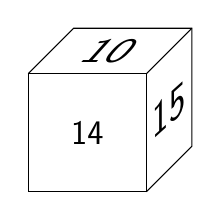
\begin{tikzpicture}[scale=0.5, every node/.style={scale=0.5}, baseline=(current bounding box.north)]
			\coordinate(A) at (0,0,0);
			\coordinate(B) at (0,3,0);
			\coordinate(C) at (3,3,0);
			\coordinate(D) at (3,0,0);
			\coordinate(E) at (0,0,3);
			\coordinate(F) at (0,3,3);
			\coordinate(G) at (3,3,3);
			\coordinate(H) at (3,0,3);

			\draw (E) -- (F) -- (G) -- (H) -- cycle;
			\draw (F) -- (B) -- (C) -- (D) -- (H);
			\draw (C) -- (G);

			\node at ($(E)!0.5!(G)$){\fontsize{64}{32}\selectfont\sf 14};
			\node[text effects={xslant=0.9}, xscale=1.4] at ($(F)!0.5!(C)$){\fontsize{40}{32}\selectfont\sf 10};
			\node [text effects={yslant=0.9}, yscale=1.4] at ($(H)!0.5!(C)$){\fontsize{36}{32}\selectfont\sf 15};
		\end{tikzpicture}
	\end{minipage}

	\begin{oneparchoices}
		\choice 78 \choice 80 \CorrectChoice 89 \choice 107 \choice 以上都不对
	\end{oneparchoices}
	\begin{solution}\\
		10、14、15三个数的最小公倍数为:210,则有
		\begin{equation*}
			\begin{cases}
				10\text{的对面是} 21 \\
				14\text{的对面是} 15 \\
				15\text{的对面是} 14
			\end{cases}
		\end{equation*}
	\end{solution}

	\question 找出下列比 \( \displaystyle \sqrt{22 + \sqrt{22 + \sqrt{22 + \sqrt{22}}}} \)小的最大整数。

	\begin{oneparchoices}
		\choice 4 \CorrectChoice 5 \choice 9 \choice 20 \choice 25
	\end{oneparchoices}
	\begin{solution}
		\begin{align*}
			\sqrt{22 + \sqrt{22 + \sqrt{22 + \sqrt{22}}}} & > \sqrt{22 + \sqrt{22 + \sqrt{22 + 4}}} \\
			                                              & > \sqrt{22 + \sqrt{22 + 5}}             \\
			                                              & > \sqrt{22 + 5}                         \\
			                                              & > 5
		\end{align*}
	\end{solution}

	\question 小明和小红正在用他们的计算器计算两个数 \( a \)和 \( b \)的平均值。首先,小明 使用计算器输入了 \( a + b
	\div 2 \) ,结果得到 \( 30 \)。然后小红使用相同的计算器输入了 \( b + a \div 2 \)结果得到 18。请问两个数的正确平均值是多少?

	\begin{oneparchoices}
		\choice 28 \choice 24 \CorrectChoice 16 \choice 12 \choice 以上都不对
	\end{oneparchoices}

	\begin{solution}
		\begin{align*}
			a    + b \div 2   & = 30 \\
			b    + a \div 2   & = 18 \\
			1.5  \times (a+b) & = 48 \\
			a    + b          & = 32 \\
		\end{align*}
		则正确的平均数为16。如果用常规的计算器是不会出现这种情况的。
	\end{solution}

	\question 下面的方程有几对整数解?
	\begin{equation}
		3x^2y - 10xy - 8y - 17 = 0
	\end{equation}
	\begin{oneparchoices}
		\choice 无 \CorrectChoice 1 \choice 2 \choice 4 \choice 以上都不对
	\end{oneparchoices}

	\begin{solution}
		\begin{align*}
			3x^2y - 10xy - 8y - 17 & = 0  \\
			y(3x^2 - 10x - 8)      & = 17 \\
			y(x-4)(3x+2)           & = 17 \\
		\end{align*}
		因为 \( 17 \) 是质数,所以只能有以下两种情况:
		\begin{equation*}
			\begin{cases}
				y = 1, \quad (x-4)(3x+2) = 17 \\
				y = 17,\quad  (x-4)(3x+2) = 1
			\end{cases}
		\end{equation*}
		在第一种情况下:
		\begin{align*}
			(x-4)(3x+2)     & = 17 \\
			3x^2 -10x - 25  & = 0  \\
			(3x + 5)(x - 5) & = 0  \\
		\end{align*}
		则 \( (x=5, y=1) \) 是方程的一组整数解。

		在第二种情况下:
		\begin{align*}
			3x^2 - 10x - 9 & = 0 \\
		\end{align*}
		此方程没有整数解。

		因此,题目中的方程只有一组整数解。
	\end{solution}

	\question 有多少个 \( n \)使得 \( \displaystyle\frac{11n+14}{n-2} \)是一个整数?

	\begin{oneparchoices}
		\choice 3 \choice 6 \choice 9 \CorrectChoice 18 \choice 以上都不是
	\end{oneparchoices}

	\begin{solution}
		\begin{equation*}
			\frac{11n + 14}{n-2} = \frac{11n - 22 + 36}{n-2} = 11 + \frac{36}{n-2}
		\end{equation*}
		\( 36 \)的因数有 \( 1,2,3,4,6,9,12,18,36 \)一共9个,再考虑到负数的情况就一共有18个了。
	\end{solution}

	\question 一枚均匀的硬币被投掷100次,结果全部是正面朝上。请问第101次投掷时,硬币正面朝上的概率是多少?

	\begin{oneparchoices}
		\choice 1 \choice \( \frac{1}{2^{100}} \) \choice \( \frac{1}{2^{101}} \) \CorrectChoice \( \frac{1}{2} \) \choice 以上都不对
	\end{oneparchoices}

	\question  如果两只土拨鼠在12分钟内可以啃掉32斤的木头,那么三只土拨鼠在8分钟内可以啃掉多少斤的木头?
	\begin{oneparchoices}
		\choice \( 21\frac13 \) \CorrectChoice 32 \choice 64 \choice 80 \choice 以上都不对
	\end{oneparchoices}

	\begin{solution}
		\begin{align*}
			32 \div 12 \div 2 \times 3 \times 8 & = \frac{32 \times 3 \times 8}{12 \times 2} \\
			                                    & = 32
		\end{align*}
	\end{solution}

	\question 假设有打呼、磨牙、抽烟三种生活不良习惯,请问下列哪个系列的前提假设能够推断出老王不喝酒?

	\begin{oneparchoices}
		\choice
		\begin{minipage}{0.25\textwidth}
			所有喝酒的人都磨牙\\
			磨牙的人不打呼 \\
			有些打呼的人抽烟 \\
			老王抽烟
		\end{minipage}
		\choice
		\begin{minipage}{0.25\textwidth}
			有些喝酒的人磨牙 \\
			没有磨牙的人会打呼 \\
			有些抽烟的人会打呼 \\
			老王抽烟
		\end{minipage}
		\choice
		\begin{minipage}{0.25\textwidth}
			所有喝酒的人磨牙 \\
			没有磨牙的人会打呼 \\
			所有打呼的人抽烟 \\
			老王抽烟
		\end{minipage}
		\CorrectChoice
		\begin{minipage}{0.25\textwidth}
			所有喝酒的人磨牙 \\
			没有磨牙的人会打呼 \\
			所有抽烟的人打呼 \\
			老王抽烟
		\end{minipage}
		\choice
		\begin{minipage}{0.25\textwidth}
			以上都不对
		\end{minipage}
	\end{oneparchoices}

	\begin{solution}

		A选项没有与喝酒相关的内容 \\
		B选项从老王抽烟与有些抽烟的人会打呼,只能推断出老王可能会打呼。
		从有些喝酒的人磨牙和没有磨牙的人会打呼,只能推断出有些喝酒的人不会打呼。\\
		C选项从老王抽烟,及所有打呼的人抽烟并不能推断出都比打呼 \\
		D选项从老王抽烟,以及所有抽烟的人打呼得出老王打呼\\
		从所有喝酒的人磨牙和没有磨牙的人会打呼得出喝酒的人不打呼,所以老王不喝酒

	\end{solution}

	\question 下列哪些表达式对于所有的 \( x \)都为 0?

	\begin{oneparchoices}
		\CorrectChoice \( (x+1)(x-1) - x^2 + 1 \)
		\choice \( x^0 - 1 \)
		\choice \( \sqrt{x^2} - x\)
		\choice 对于所有 \( x \)没有表达式的值为0
		\choice 对于所有 \( x \)有不止一个表达式值为0
	\end{oneparchoices}

	\begin{solution}
		\begin{itemize}
			\item \( (x+1)(x-1) - x^2 + 1  = x^2 - 1 - x^2 + 1 = 0  \)
			\item \( x^0 - 1 \),当 \( x=0 \)时 \( x^0 \)无定义
			\item \( \sqrt{x^2} - x = \pm x - x = 0 \,\text{或} -2x \)
		\end{itemize}
	\end{solution}

	\question 一个等边三角形的基点位于一个半径为2的圆边上,这个三角形的面积是:

	\begin{oneparchoices}
		\CorrectChoice \( 3\sqrt{3} \) \choice \( 2\sqrt{3} \) \choice \( 5\sqrt{3} \) \choice \( 4\sqrt{3} \) \choice
		以上都不是
	\end{oneparchoices}

	\begin{solution}
		\begin{center}
			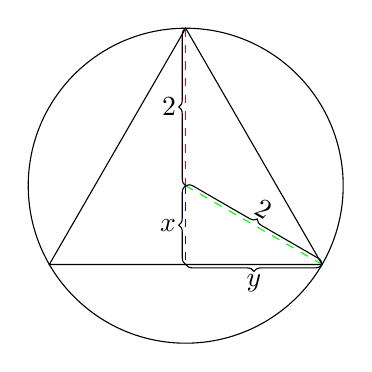
\begin{tikzpicture}
				\draw circle (2);
				\draw (90:2) -- (210:2) -- (330:2) -- cycle;
				\draw[dashed, red] (90:2) --node[anchor=east, black]{2} (0,0);
				\draw[decoration={brace, mirror}, decorate] (90:2) -- (0,0);
				\draw[dashed, green] (0,0)--node[black, sloped, above]{2} (330:2);
				\draw[decoration={brace}, decorate] (0,0)-- (330:2);
				\draw[dashed, blue] (0,0) --node[anchor=east, black]{$x$} ($(210:2)!0.5!(330:2)$);
				\draw[decoration={brace, mirror}, decorate] (0,0) -- ($(210:2)!0.5!(330:2)$);
				\draw[decoration={brace, mirror}, decorate] ($(210:2)!0.5!(330:2)$) --node[below]{$y$} (330:2);
			\end{tikzpicture}
		\end{center}

		因为是等边三角形,所以得 \( x = 1 \),所以 \( y = \sqrt{2^2 - 1^2} = \sqrt{3} \),则三角形的面积为
		\[
			2y \cdot (2 + x) / 2=  3\sqrt{3}
		\]
	\end{solution}

	\question 存在多少个仅由0和1组成的7位数能够被6整除?

	\begin{oneparchoices}
		\choice 10 \CorrectChoice 11 \choice 16 \choice 21 \choice 33
	\end{oneparchoices}

	\begin{solution}
		首先,末位必须是0以保证能被2整除。前面的6位要能被3整除,则数字和为3的倍数。
		\begin{enumerate}
			\item 数字和为6的话,只有一种情况。
			\item 数字和为3的话,最左边一位必须是1
			      \begin{equation*}
				      \binom{5}{2} = \frac{5!}{2!(5-2)!} = \frac{5 \times 4 \times 3}{3 \times 2 \times 1} = 10
			      \end{equation*}
		\end{enumerate}
		所以一共有11个符合条件的整数。
	\end{solution}

	\question 假设 \( x \)和 \( y \)满足 \( \frac{x-y}{x+y}=9 \)和 \( \frac{xy}{x+y}=-60 \),那么 \( (x+y) + (x-y) + xy
	\)的值是?

	\begin{oneparchoices}
		\choice \( -50 \) \CorrectChoice \( -150 \) \choice \( -14310 \) \choice 210 \choice 14160
	\end{oneparchoices}

	\begin{solution}
		\begin{align*}
			(x+y) + (x-y) + xy & = (x+y) + 9(x+y) -60(x+y) \\
			                   & = -50(x+y)
		\end{align*}
		设 \( a = x + y, a \ne 0 \),则
		\begin{align*}
			a^2         & = (x+y)^2              \\
			            & = x^2 + 2xy + y^2      \\
			            & = x^2 - 2xy + y^2 +4xy \\
			            & = (x-y)^2 + 4xy        \\
			            & = (9a)^2 + 4(-60a)     \\
			80a^2 -240a & = 0                    \\
		\end{align*}
		因为 \( a \ne 0 \),所以 \( a = 3 \),则原式等于 \( -150 \)。
	\end{solution}

	\question 一个圆周上等距离地分布着 \( n \)个点,并且按照顺序用整数 \( 1 \)到 \( n
	\)进行标记。如果两个点通过圆的直径连接,我们称这两个点是相对的。如果标记为 \( 7 \)和 \( 35 \)的点是相对的,那么 \( n \)等于多少?

	\begin{oneparchoices}
		\choice 54 \choice 55 \CorrectChoice 56 \choice 57 \choice 以上都不对
	\end{oneparchoices}

	\begin{solution}
		因为7和35的点是相对的,那么在7和35连成的直径两边各有 \( 34 - 7 = 27 \)个点,再加上本身的两个,一共是56个点。
	\end{solution}

	\question 一个菱形的边长是10 cm,并且两条对角线的差是4 cm,那么这个菱形的面积是多少?

	\begin{oneparchoices}
		\CorrectChoice \( 96\, \text{cm}^2 \) \choice \( 100\, \text{cm}^2 \) \choice \( 100\sqrt{2}\, \text{cm}^2 \) \choice
		信息不够 \choice 以上都不对
	\end{oneparchoices}

	\begin{solution}\\
		\begin{minipage}{0.4\textwidth}
			\begin{tikzpicture}[scale=0.5, baseline = (current bounding box.north)]
				\coordinate (A) at (0,5);
				\coordinate (B) at (3,0);
				\coordinate (C) at (0,-5);
				\coordinate (D) at (-3,0);
				\node [shape=diamond, draw, minimum width=6cm, minimum height=10cm, scale=0.5](x){};
				\node[above] at (A) {A};
				\node[right] at (B) {B};
				\node[below] at (C) {C};
				\node[left] at (D) {D};
				\draw[dashed, name path=AC] (A) -- (C);
				\draw[dashed, name path=BD] (B) -- (D);
				\path[name intersections={of=AC and BD, by={O}}];
				\node[below right] at (O) {O};
			\end{tikzpicture}
		\end{minipage}
		\begin{minipage}{.5\textwidth}
			\begin{equation*}
				AC - BD  = 4
			\end{equation*}
			则
			\begin{equation*}
				OC - OB  = 2
			\end{equation*}
			设 \( OB = x \),则有
			\begin{align*}
				x^2 + (2+x)^2     & = 10^2 \\
				x^2 + x^2 + 4x +4 & = 100  \\
				x^2 +2x -48       & = 0    \\
				(x-6)(x+8)        & = 0    \\
				x                 & = 6
			\end{align*}
			则 \( OC = 8 \), 菱形的面积为 \( 6 \times 8 \div 2 \times 4 = 96\, \text{cm}^2 \)
		\end{minipage}
	\end{solution}

	\question \( P \)点在一个边长是2的等边三角形之内, \( P \)点到三个顶点的距离分别是 \( x, y \)和 \( z \),那么 \( x +
	y + z \)等于多少?

	\begin{oneparchoices}
		\CorrectChoice \( \sqrt{3} \) \choice \( 2\sqrt{3} \) \choice \( 3\sqrt{3} \) \choice 条件不足 \choice 以上都不对
	\end{oneparchoices}

	\begin{solution}\\
		\begin{minipage}{0.49\textwidth}
			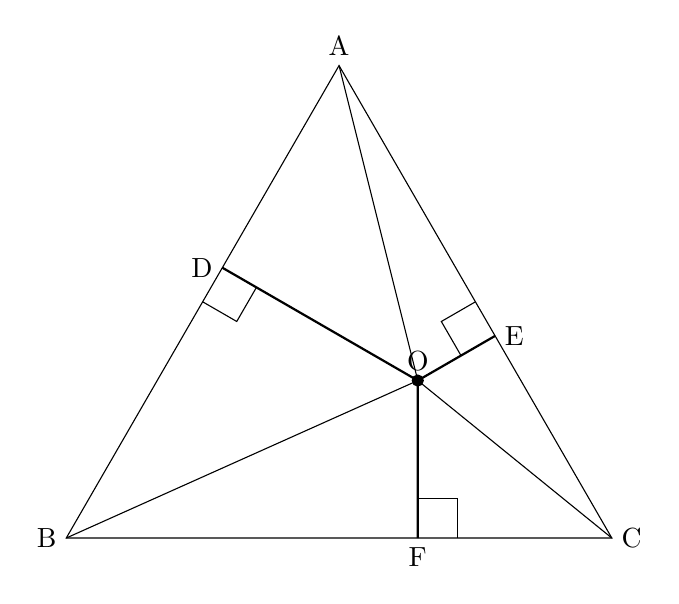
\begin{tikzpicture}[scale=2]
				\coordinate (A) at (90:2);
				\coordinate (B) at (210:2);
				\coordinate (C) at (330:2);
				\coordinate (O) at (0:.5);
				\coordinate (D) at ($(A)!(O)!(B)$);
				\coordinate (E) at ($(C)!(O)!(A)$);
				\coordinate (F) at ($(B)!(O)!(C)$);
				\draw (A)node[above]{A} -- (B)node[left]{B} -- (C)node[right]{C} -- cycle;
				\draw[fill] (O) circle[radius=1pt];
				\node[above] at (O) {O};
				\node[left] at (D) {D};
				\node[right] at (E) {E};
				\node[below] at (F) {F};
				\pic[draw]{right angle = B--D--O};
				\pic[draw]{right angle = A--E--O};
				\pic[draw]{right angle = C--F--O};
				\draw[thick] (O) -- ($(B)!(O)!(C)$) (O) -- ($(A)!(O)!(B)$) (O) -- ($(A)!(O)!(C)$);
				\draw (A) -- (O) (B) -- (O) (C) -- (O);
			\end{tikzpicture}
		\end{minipage}
		\begin{minipage}{0.5\textwidth}
			\begin{align*}
				A_{\triangle{ABC}} & = \frac12 \times 2 \times \sqrt{3}                               \\
				                   & = \sqrt{3}                                                       \\
				                   & = A_{\triangle{AOC}} + A_{\triangle{BOC}} + A_{\triangle{AOB}}   \\
				                   & = \frac12 AC\cdot OE + \frac12 BC \cdot OF + \frac12 AB \cdot OD \\
				                   & = OE + OF + OD
			\end{align*}
			所以 \( x + y + z \)值为 \( \sqrt3 \)
		\end{minipage}
	\end{solution}
	\question 一个矩形的的长为 \( l \)宽为 \( w \),且有 \( l > w \)。 对其中一个值增长 \( 20\% \),另一个减小 \( 20\%
	\),矩形的面积会发生怎样的变化?

	\begin{oneparchoices}
		\choice 不变 \CorrectChoice 减小 \choice 变大 \choice 只有当 \( l \)增长时才变大 \choice 只有当 \( w \)增长时才变大
	\end{oneparchoices}

	\begin{solution}
		假设 \( l \)增大 \( 20\% \),而 \( w \)减小 \( 20\% \),则面积变为 \( 1.2l \cdot 0.8w = 0.96lw \)

		同样的,如果 \( l \)减小 \( 20\% \)而 \( w \)增大 \( (20\%) \)可以计算出变化后的面积也是 \( 0.96lw
		\),所以面积会减小。
	\end{solution}

\end{questions}
\end{document}

%!tex program = lualatex
\documentclass[answers]{exam}
\usepackage{ctex}
\usepackage{graphicx}
\usepackage[margin=2cm]{geometry}
\usepackage{amsmath, amssymb}
\usepackage{csquotes}
\usepackage{tikz, pgfplots}
\usetikzlibrary{
	angles,
	backgrounds,
	calc,
	decorations.pathmorphing,
	decorations.pathreplacing,
	decorations.text,
	intersections,
	patterns,
	quotes,
	shapes,
	shapes.symbols,
}
\pagestyle{empty}
\newcounter{xcord}
\newcounter{ycord}
\newcounter{total}
\renewcommand{\labelenumi}{\textbf{\ifnum\value{enumi}<10 0\fi\arabic{enumi})}}

\pgfplotsset{compat=1.18}

\CorrectChoiceEmphasis{\color{blue!70!green}\bfseries}
\renewcommand{\solutiontitle}{\textbf{解:}}

\usepackage{array, tabularx}
\newcolumntype{C}{>{\centering\arraybackslash}X}
\newcolumntype{B}{>{\centering\bfseries\arraybackslash}X}
\catcode`\幺=0

\begin{document}
\begin{questions}
	\question 对于 \( n \ge 2 \),让 \( k_n = 5 \cdot 10 \cdot 17 \cdot 26 \cdot\cdots\cdot (n^2 + 1) \),
	\begin{equation*}
		S_n = (1-\frac{1}{2^4})(1-\frac{1}{3^4})\cdots(1-\frac{1}{n^4}).
	\end{equation*}
	那么 \( S_n / k_n \)等于:

	\begin{oneparchoices}
		\CorrectChoice \(\displaystyle \frac{1}{2}\frac{1}{(n!)^2}(1+\frac{1}{n}) \)
		\choice \(\displaystyle \frac{1}{k_n}\frac{n^2}{n^4 + 1} \)
		\choice \(\displaystyle \frac{n^4 + 1}{2n+2}\cdot \frac{1}{n!} \)
		\choice \(\displaystyle \frac{1}{k_n}\frac{1}{n^4}\frac{1}{((n-1)!)^4} \)
		\choice 以上都不对
	\end{oneparchoices}

	\begin{solution}
		\begin{align*}
			S_n / k_n & = \frac{(1-\frac{1}{2^4})(1-\frac{1}{3^4})\cdots(1-\frac{1}{n^4})}{5 \cdot 10 \cdot 17 \cdot 26
			\cdot\cdots\cdot (n^2 + 1)}                                                                                 \\
			          & = \prod_2^n\frac{1 - \frac{1}{n^4}}{n^2 + 1}                                                    \\
			          & = \prod_2^n\frac{n^4 - 1}{n^4(n^2+1)}                                                           \\
			          & = \prod_2^n\frac{n^2 - 1}{n^4}                                                                  \\
			          & = \prod_2^n\frac{1 - \frac{1}{n^2}}{n^2}                                                        \\
			          & = \frac{1}{(n!)^2} \prod_2^n(1-\frac{1}{n^2})                                                   \\
			          & = \frac{1}{(n!)^2} \prod_2^n\frac{(n-1)(n+1)}{n^2}                                              \\
			          & = \frac{1}{(n!)^2} \frac{(2-1)(2+1)(3-1)(3+1)\cdots
			(n-3)(n-1)(n-2)n(n-1)(n+1)}{2^2\cdot3^2\cdots (n-1)^2n^2}                                                   \\
			          & = \frac{1}{(n!)^2} \frac{1\cdot2\cdot 3^2 \cdot 4^2 \cdots (n-1)^2 \cdot n \cdot
			(n+1)}{2^2\cdot3^2\cdots (n-1)^2\cdot n^2}                                                                  \\
			          & = \frac{1}{(n!)^2} \frac{2n(n+1)}{2^2\cdot n^2}                                                 \\
			          & = \frac12\frac1{(n!)^2}(1+\frac1n)
		\end{align*}
	\end{solution}

	\question 下列选项中,哪个不是方程:
	\begin{equation*}
		3^x - 6^x = 12^x - \left(\frac32\right)^x.
	\end{equation*}
	的解?

	\begin{oneparchoices}
		\choice \( \dfrac{3\pi i}{\ln2} \)
		\choice 0
		\choice \( \dfrac{6\pi i}{\ln2} \)
		\choice \( \dfrac{27\pi i}{\ln2} \)
		\CorrectChoice 所有都是解
	\end{oneparchoices}

	\begin{solution}
		\begin{align*}
			3^x - 6^x                               & = 12^x - \left(\frac32\right)^x             \\
			3^x - 2^x \cdot 3^x                     & = 2^x \cdot 2^x \cdot 3^x - \frac{3^x}{2^x} \\
			2^x \cdot 3^x - 2^x \cdot 2^x \cdot 3^x & = 2^x \cdot 2^x \cdot 2^x \cdot 3^x - 3^x
		\end{align*}
		设 \( a = 2^x, b = 3^x \),则有
		\begin{align*}
			a^3b + a^2b - ab - b & = 0
		\end{align*}
		因为 \( b \ne 0 \),所以进一步化简得
		\begin{align*}
			a^3 + a^2 - a - 1 & = 0 \\
			a^2(a+1) - (a+1)  & = 0 \\
			(a+1)(a^2 - 1)    & = 0 \\
			(a+1)^2(a-1)      & = 0
		\end{align*}
		则有 \( a = \pm 1 \)即 \( 2^x = \pm 1 \)

		欧拉公式 \( e^{i\theta} = \cos\theta + i\sin\theta \)对于 \( \theta = k\pi, k \in \mathbb{Z}  \)时有
		\begin{equation*}
			\begin{cases}
				\cos(k\pi) + i\sin(k\pi) = 1, k \text{是偶数} \\
				\cos(k\pi) + i\sin(k\pi) = -1, k \text{是奇数}
			\end{cases}
		\end{equation*}
		将 \( 2^x = e^{x\ln2} \)代入欧拉公式有
		\begin{gather*}
			x \ln 2 = k\pi i,  k \in \mathbb{Z} \\
			x = \frac{k\pi i}{\ln2}, k \in \mathbb{Z}
		\end{gather*}
		所以选E
	\end{solution}

	\question 考虑方程$p(x): ax^2 + bx + c=0$,其系数$a$,$b$和$c$都是非零的,并且每个系数都满足从方程$p(x)$
	中移除包含该系数的项后得到的方程;例如,系数$b$是方程 $ax^2+c=0$的一个解。求方程$p(x)$
	所有解的和是多少?

	\begin{oneparchoices}
		\choice 总是 1 \choice 总是 -1 \choice 总是 2 \CorrectChoice 1 或者 -1 \choice 1 或者 2
	\end{oneparchoices}
	\begin{solution}
		方程$p(x)$的两个解分别为$\displaystyle x_1, x_2 = \frac{-b \pm \sqrt{b^2 - 4ac}}{2a}$,则$\displaystyle x_1 +
			x_2 = -\frac{b}{a}$\\
		由题意得
		\begin{align}
			ac^2  + bc & = 0 \label{\thequestion:1} \\
			ab^2  + c  & = 0 \label{\thequestion:2} \\
			ab    + c  & = 0 \label{\thequestion:3}
		\end{align}
		由式(\ref{\thequestion:2}) 和(\ref{\thequestion:3})得$b=1$和$a+c=0$,代入(\ref{\thequestion:1})得:
		\begin{equation}
			a(-a)^2 -a  = 0
		\end{equation}

		则$a=\pm 1$或$a=0$,因为题目中$a \ne 0$,所以$a=\pm 1$,则$\displaystyle x_1 + x_2 = -\frac{b}{a}=\pm 1$

		此题与2022level1中重复
	\end{solution}

	\question 求下列序列前五项的和:
	\begin{equation*}
		\left\{ \dfrac{2}{3}, \dfrac{4}{9}, \dfrac{8}{27}, \dots\right\}
	\end{equation*}

	\begin{oneparchoices}
		\choice \( \dfrac{64}{81} \)
		\choice \( \dfrac{550}{243} \)
		\choice \( \dfrac{32}{81} \)
		\CorrectChoice \( \dfrac{422}{243} \)
		\choice 以上都不对
	\end{oneparchoices}

	\begin{solution}
		设 \( S_5 = \dfrac{2}{3} + \left(\dfrac{2}{3}\right)^2 + \dots + \left(\dfrac{2}{3}\right)^5\)
		则有
		\begin{align*}
			\dfrac{2}{3}\cdot S_5 & = \left(\dfrac{2}{3}\right)^2 + \dots + \left(\dfrac{2}{3}\right)^6 \\
			\dfrac{1}{3}\cdot S_5 & = \dfrac{2}{3} - \left(\dfrac{2}{3}\right)^6                        \\
			S_5                   & = 2 - \dfrac{2^6}{3^5}                                              \\
			                      & = \dfrac{243 \times 2 - 64}{243}                                    \\
			                      & = \dfrac{422}{243}
		\end{align*}
	\end{solution}

	\question 假设 \( f \)是一个函数,并有 \( f(n+1) = f(n) + 3f(n-1) \)对所有整数成立。如果 \( f(4) = 151 \)和 \( f(1)
	= 1\),那么 \( f(-1) \)的值是多少?

	\begin{oneparchoices}
		\choice 12 \choice 4 \CorrectChoice \( -\dfrac{11}{3} \) \choice \( \dfrac{13}{3} \) \choice 以上都不对
	\end{oneparchoices}

	\begin{solution}
		由题意得
		\begin{align*}
			f(4)  & = f(3) + 3f(2)           \\
			f(3)  & = f(2) + 3f(1)           \\
			f(4)  & = f(2) + 3f(1) + 3f(2)   \\
			151   & = 4f(2) + 3              \\
			f(2)  & = \dfrac{151 -3}{4} = 37 \\
			      & = f(1) + 3f(0)           \\
			f(0)  & = 12                     \\
			f(1)  & = f(0) + 3f(-1)          \\
			f(-1) & = -\dfrac{11}{3}
		\end{align*}
	\end{solution}

	\question 对下式进行分母有理化
	\begin{equation*}
		\dfrac{1}{2^{5/6} + 2^{1/2} + 2^{1/3} + 1}
	\end{equation*}

	\begin{oneparchoices}
		\choice \( \dfrac{1}{6}(2^{1/2} + 2^{1/3} - 2^{1/6}) \)
		\choice \( \dfrac{1}{3}(2^{1/2} - 1)(2^{2/3} - 2^{1/3} + 1) \)
		\choice \( \dfrac{1}{2}(2^{7/6} - 2^{5/6} + 1) \)
		\CorrectChoice \( (2^{1/2} - 1)(2^{2/3} - 2^{1/3} + 1) \)
		\choice 以上都不对
	\end{oneparchoices}

	\begin{solution}
		\begin{align*}
			\dfrac{1}{2^{5/6} + 2^{1/2} + 2^{1/3} + 1} & = \dfrac{1}{(2^{1/6})^5 + (2^{1/6})^3 + (2^{1/6})^2 + 1},
			\qquad \text{设} a = 2^{1/6}                                                                              \\
			                                           & = \dfrac{1}{a^5 + a^3 + a^2 + 1}                             \\
			                                           & = \dfrac{1}{a^3(a^2 + 1) + a^2 + 1}                          \\
			                                           & = \dfrac{1}{(a^3 + 1)(a^2 + 1)}                              \\
			                                           & = \dfrac{a^3 - 1}{(a^6 - 1)(a^2 + 1)}                        \\
			                                           & = \dfrac{a^3 - 1}{a^2 + 1}                                   \\
			                                           & = \dfrac{(a^3 - 1)(a^4 - a^2 + 1)}{(a^2 + 1)(a^4 - a^2 + 1)} \\
			                                           & = (a^3 - 1)(a^4 - a^2 + 1)                                   \\
			                                           & = (2^{1/2} - 1)(2^{2/3} - 2^{1/3} + 1)
		\end{align*}
	\end{solution}

	\question 求\(  \displaystyle\sum_{k=0}^{2022}\frac{2022!\cdot (-1)^k2^k}{k! \cdot (2022-k)!}\) 的值

	\begin{oneparchoices}
		\choice \( \dfrac{1-(-2)^{2023}}{3} \)
		\choice -1
		\CorrectChoice 1
		\choice \( 3^{2022} \)
		\choice 以上都不对
	\end{oneparchoices}

	\begin{solution}
		\begin{enumerate}
			\item 利用二项式定理$\displaystyle(x+y)^n = \sum_{k=0}^{n}\binom{n}{k}x^ky^{n-k}$
			      \begin{align*}
				      \sum_{k=0}^{2022}\frac{2022!\cdot(-1)^k2^k}{k!\cdot(2022-k)!} & = \sum_{k=0}^{2022}\frac{2022!}{k!\cdot
				      (2022-k)!}(-2)^k                                                                                        \\
				                                                                    & =
				      \sum_{k=0}^{2022}\binom{2022}{k}(-2)^k\cdot 1^{2022-k}                                                  \\
				                                                                    & = (1-2)^{2022}                          \\
				                                                                    & = 1
			      \end{align*}
		\end{enumerate}
	\end{solution}

	\question $(\sqrt[4]{27} + \sqrt{3} + \sqrt[4]{3} + 1)^2$ 与下列哪个相等

	\begin{oneparchoices}
		\CorrectChoice \( \dfrac{4}{\sqrt{3} - 2\sqrt[4]{3} + 1} \)
		\choice \( 4\sqrt{3} + 4 \)
		\choice \( 2\sqrt[4]{27} + 2\sqrt[4]{3} + 6\sqrt{3} + 6 \)
		\choice \( \dfrac{16}{\sqrt{3} + 2\sqrt[4]{3} + 1} \)
		\choice 以上都不对
	\end{oneparchoices}

	\begin{solution}
		\begin{enumerate}
			\item 设$\displaystyle x=3^{\frac{1}{4}}$,则
			      \begin{align*}
				      (\sqrt[4]{27} + \sqrt{3} + \sqrt[4]{3} + 1)^2 & = (x^3 + x^2 + x + 1)^2                     \\
				                                                    & = [x^2(x+1) + (x+1)]^2                      \\
				                                                    & = (x^2 + 1)^2(x+1)^2                        \\
				                                                    & = \frac{(x^2 + 1)^2(x+1)^2(x-1)^2}{(x-1)^2} \\
				                                                    & = \frac{(x^4 - 1)^2}{(x-1)^2}
			      \end{align*}
			\item 将$x=\sqrt[4]{3}$代入得:
			      \begin{align*}
				      \frac{(x^4 - 1)^2}{(x-1)^2} & = \frac{4}{(x-1)^2}                     \\
				                                  & = \frac{4}{x^2 - 2x + 1}                \\
				                                  & = \frac{4}{\sqrt{3} - 2\sqrt[4]{3} + 1}
			      \end{align*}
		\end{enumerate}
	\end{solution}

	\question 哪个选项与以下表达式相等:

	\begin{equation*}
		\dfrac{(3x+2)^{\frac{1}{2}}\left(\frac{1}{3}\right)(2x+3)^{-\frac{2}{3}}(2) -
		(2x+3)^{\frac{1}{3}}\left(\frac{1}{2}\right)(3x+2)^{-\frac{1}{2}}(3)}{\left[(3x+2)^\frac{1}{2}\right]^2}
	\end{equation*}

	\begin{oneparchoices}
		\choice \(  \dfrac{-5}{6(2x+3)^{\frac{4}{3}}(3x+2)^2}\)
		\choice \( \dfrac{2\sqrt{3x+2} - 3\sqrt[3]{2x+3}}{6\sqrt{(3x+2)^3}\sqrt[3]{(2x+3)^2}} \)
		\choice 0
		\CorrectChoice \( -\dfrac{6x+19}{6(2x+3)^{\frac{2}{3}}(3x+2)^{\frac{3}{2}}} \) \\
		\choice 以上都不对
	\end{oneparchoices}

	\begin{solution}
		设 \( a = (3x + 2)^{\frac12}, b = (2x + 3)^{\frac13} \),则有
		\begin{align*}
			\dfrac{\frac23ab^{-2} - \frac32a^{-1}b}{a^2} & = \dfrac{4a^2b^{-2} - 9b}{6a^3}                                 \\
			                                             & = \dfrac{4a^2 - 9b^3}{6a^3b^2}                                  \\
			                                             & = \dfrac{4(3x+2) - 9(2x +3)}{6(3x+2)^{\frac32}(2x+3)^{\frac23}} \\
			                                             & = \dfrac{12x + 8 - 18x - 27}{6(3x+2)^{\frac32}(2x+3)^{\frac23}} \\
			                                             & = \dfrac{-6x - 19}{6(3x+2)^{\frac32}(2x+3)^{\frac23}}
		\end{align*}
	\end{solution}

	\question
	一个人沿着海滩走,从点A开始,以每小时3公里的速度行走,并且在B点进入水中,以每小时2公里的速度斜向游到一个距离C点$\sqrt{3}$公里远的小岛上,直接横跨岛屿与海岸线相对的位置,如图所示。从A点到C点的总距离为3公里。有两种不同的选择,从A点到B点的距离(以公里为单位)将导致步行和游泳的总时间为一小时四十分钟;这两个数字之和是多少?

	\begin{oneparchoices}
		\choice 2 \choice 4 \CorrectChoice $\frac{14}{5}$ \choice $\frac{16}{5}$ \choice 以上都不对
	\end{oneparchoices}

	\begin{figure}[ht]
		\centering
		\begin{tikzpicture}[scale=0.8, every node/.style={transform shape}]
			% Define coordinates
			\coordinate (A) at (0,0);
			\coordinate (B) at (2,0);
			\coordinate (C) at (3,0);
			\coordinate (D) at (3,{sqrt(3)});

			% Draw horizontal lines for the sea
			\begin{scope}[on background layer]
				\draw[dashed] (A) -- (B);
				\draw[dashed] (B) -- (C);
				\draw[dashed] (C) -- (D);
				\draw[dashed] (B) -- (D);
			\end{scope}

			\node[fill=white] at (A){$A$};
			\node[fill=white] at (B){$B$};
			\node[fill=white] at (C){$C$};
			\node[cloud, draw=black, minimum width=3cm, minimum height=2cm, anchor=south] at (D){小岛};

			\draw[decoration={coil, segment length = 5mm, amplitude = 0.5mm}, decorate] ([yshift=0.5cm]A) -- ([yshift=0.5cm]C);
			\draw[decoration={brace, mirror}, decorate] ([yshift=-0.5cm]A) -- ([yshift=-0.5cm]C);
			\draw[decoration={brace, mirror}, decorate] ([xshift=0.5cm]C) -- ([xshift=0.5cm]D);
			\node at ([yshift=-1cm]$(A)!0.5!(C)$) {3公里};
			\node at ([xshift=1.5cm]$(C)!0.5!(D)$) {$\sqrt{3}$公里};

			\node at (0,2) {\~{}};
			\node at (1,1.5) {\~{}};
			\node at (2,1) {\~{}};
			\node at (2,1.5) {\~{}};

		\end{tikzpicture}
		\caption{\thequestion}
	\end{figure}

	\begin{solution}
		\begin{enumerate}
			\item 设$AB=x$,则$BC=3-x$
			\item 设$B$点到小岛的距离为$y$,则有
			      \begin{equation*}
				      y^2 = (3-x)^2 + 3 \label{\thequestion:step2}
			      \end{equation*}
			\item 根据总时间可以得
			      \begin{gather*}
				      \frac{x}{3} + \frac{y}{2} = \frac{100}{60} = \frac{5}{3}\\
				      2x + 3y = 10 \\
				      y = \frac{10 - 2x}{3}
			      \end{gather*}
			\item 将$y$代入式(\ref{\thequestion:step2})中,得
			      \begin{gather*}
				      \frac{(10-2x)^2}{3^2} = 9 - 6x + x^2 + 3 \\
				      100 -40x + 4x^2 = 108 - 54x + 9x^2 \\
				      5x^2 -14x + 8 = 0 \label{\thequestion:step4}
			      \end{gather*}
			\item 方程(\ref{\thequestion:step4})的两个解的和
			      \begin{equation*}
				      x_1 + x_2 = \frac{-(-14) \times 2}{5 \times 2} = \frac{14}{5}
			      \end{equation*}
		\end{enumerate}
	\end{solution}

	\question 哪个选项是以下不等式的解?
	\begin{equation*}
		\dfrac{1}{|x-3|} + \dfrac{2}{x-3} \le 5
	\end{equation*}

	\begin{oneparchoices}
		\CorrectChoice \( (-\infty, 3) \cup \left[\frac{18}{5}, \infty\right)\)
			\choice \( \left(-\infty, \frac{16}{5}\right] \cup \left[\frac{18}{5}, \infty\right)\)
			\choice \( (-\infty, 3] \cup \left[\frac{18}{5}, \infty\right)\)
		\choice \( \left[ \frac{16}{5}, \frac{18}{5}\right] \)
		\choice 以上都不对
	\end{oneparchoices}

	\begin{solution}
		\begin{enumerate}
			\item \( x > 3 \)
			      \begin{align*}
				      \dfrac{1}{|x-3|} + \dfrac{2}{x-3}   & \le 5             \\
				      \dfrac{1}{x - 3} + \dfrac{2}{x - 3} & \le 5             \\
				      3                                   & \le 5(x-3)        \\
				      x                                   & \ge \dfrac{18}{5} \\
			      \end{align*}
			      \( x \ge \dfrac{18}{5} \) 的范围比 \( x > 3 \)小,所以取 \( x \ge \dfrac{18}{5} \)。
			\item \( x < 3 \)
			      \begin{align*}
				      \dfrac{1}{|x-3|} + \dfrac{2}{x-3} & \le 5             \\
				      -\dfrac{1}{x-3} + \dfrac{2}{x-3}  & \le 5             \\
				      \dfrac{1}{x-3}                    & \le 5             \\
				      \text{因为} x - 3 < 0, \text{所以}                   \\
				      1                                 & \ge 5(x - 3)      \\
				      x                                 & \le \dfrac{16}{5}
			      \end{align*}
			      因为 \( x < 3 \)的范围比 \( x < \dfrac{16}{5} \)小,所以取 \( x < 3 \)
		\end{enumerate}
	\end{solution}

	\question 一个游戏包含一组三个均匀的六面骰子。在其中的一组骰子中,有两个是正常的,标有数字1到6,而由于制造错误,第三个骰子的原本应该标有1的那一面被错误地标成了6(所以这个骰子上有两个面标有6)。假设从这三个骰子中随机选择两个,并掷一次。求这两个骰子都显示6点朝上的概率是多少?

	\begin{oneparchoices}
		\CorrectChoice \( \frac{5}{108} \)
		\choice \( \frac{1}{24} \)
		\choice \( \frac{1}{18} \)
		\choice \( \frac{1}{6} \)
		\choice 以上都不对
	\end{oneparchoices}

	\begin{solution}
		从三个骰子中随机挑选两个,一共有三种情况,其中有两种有有问题的骰子。所以有问题的骰子参与的概率是 \( \frac{2}{3} \)。两个正常骰子都是6点的概率是 \( \frac{1}{36}
		\),一个正常骰子与有问题的骰子都是6点的概率是 \( \frac{1}{18} \),有问题的骰子被挑中的机率是 \( \frac{2}{3}
		\),则在有问题骰子被选中的情况下,出现两个6点的概率是 \( \frac{2}{3} \times \frac{1}{18} = \frac{1}{27} \)。另外,还有 \(
		\frac{1}{3} \)的机率是两个正常的骰子被选中,这种情形下出现两个6点的机率是 \( \frac{1}{3} \times \frac{1}{36} =
		\frac{1}{108} \),两种情况加起来一共是 \( \frac{5}{108} \)
	\end{solution}

	\question 求值 \( (1+i)^{2022} \)。

	\begin{oneparchoices}
		\choice 1
		\CorrectChoice \( -2^{1011}i \)
		\choice \( 2^{1011}i \)
		\choice \( 1011 - 2022i \)
		\choice 以上都不对
	\end{oneparchoices}

	\begin{solution}
		\begin{align*}
			(1 + i) ^ {2022} & = [(1+i)^2]^{1011}    \\
			                 & = (2i)^{1011}         \\
			                 & = 2^{1011}(-1)^{505}i \\
			                 & = -2^{1011}i
		\end{align*}
	\end{solution}

	\question 下列哪个等于 \(\displaystyle \sin\left(\frac{\pi}{8}\right) \)?

	\begin{oneparchoices}
		\choice \(\displaystyle \sqrt{\frac{2-\sqrt{2}}{2}} \)
		\choice \(\displaystyle \sqrt{\frac{2+\sqrt{2}}{2}} \)
		\CorrectChoice \(\displaystyle \frac{\sqrt{2-\sqrt{2}}}{2} \)
		\choice \(\displaystyle \frac{\sqrt{2+\sqrt{2}}}{2} \)
		\choice 以上都不对
	\end{oneparchoices}

	\begin{solution}
		\begin{align*}
			\text{根据欧拉公式} e^{i\theta} & = \cos\theta + i\sin\theta,
			\quad\text{将}\theta = \frac{\pi}{8} \text{代入得}                                                   \\
			e^{\frac{\pi}{8}i}              & =
			\cos\left(\frac{\pi}{8}\right) + \sin\left(\frac{\pi}{8}\right)i,\quad \text{记作}z                  \\
			z^2                             & = e^{\frac{\pi}{4}i}
			= \left(\cos\frac{\pi}{8}\right)^2 - \left(\sin\frac{\pi}{8}\right)^2 +
			2\sin\left(\frac{\pi}{8}\right)\cos\left(\frac{\pi}{8}\right)i                                       \\
			                                & = \cos\left(\frac{\pi}{4}\right) + \sin\left(\frac{\pi}{4}\right)i \\
			                                & = \frac{\sqrt{2}}{2} + \frac{\sqrt{2}}{2}i                         \\
		\end{align*}
		则有:
		\begin{equation*}
			\begin{cases}
				\left(\cos\frac{\pi}{8}\right)^2 - \left(\sin\frac{\pi}{8}\right)^2  = \frac{\sqrt{2}}{2} \\
				2\sin\left(\frac{\pi}{8}\right)\cos\left(\frac{\pi}{8}\right) = \frac{\sqrt{2}}{2}
			\end{cases}
		\end{equation*}
		将 \(\displaystyle \cos\left(\frac{\pi}{8}\right) = \frac{\sqrt{2}}{4\sin\left(\frac{\pi}{8}\right)}\)代入得
		\[
			\left(\frac{\sqrt{2}}{4\sin\left(\frac{\pi}{8}\right)}\right)^2 - \left(\sin\frac{\pi}{8}\right)^2  = \sqrt{2}
		\]
		设 \( \sin\left(\frac{\pi}{8}\right) = a \),则有
		\begin{align*}
			\frac{1}{8a^2} - a^2 & = \frac{\sqrt{2}}{2}                       \\
			1 - 8a^4             & = 4\sqrt{2}a^2                             \\
			a^2                  & = \frac{-4\sqrt{2} \pm \sqrt{32 + 32}}{16} \\
			                     & = \frac{-\sqrt{2} \pm 2}{4}                \\
			\text{因为}a^2 \ge 0 \text{有}\quad
			a^2                  & = \frac{2-\sqrt{2}}{4}                     \\
			\text{因为} a > 0 \quad
			a                    & = \frac{\sqrt{2-\sqrt{2}}}{2}
		\end{align*}

		\begin{itemize}
			\item 三角恒等式:
			      \begin{equation}
				      \sin^2(\theta) +\cos^2(\theta) = 1
			      \end{equation}
			\item 和角公式
			      \begin{gather}
				      \sin(\alpha + \beta) = \sin\alpha\cos\beta + \sin\beta\cos\alpha \\
				      \cos(\alpha + \beta) = \cos\alpha\cos\beta - \sin\alpha\sin\beta
			      \end{gather}
			      \clearpage
			      \begin{minipage}{0.53\textwidth}
				      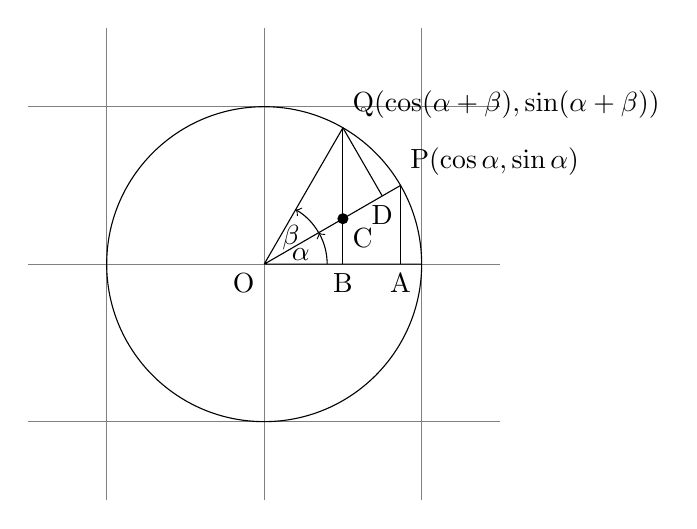
\begin{tikzpicture}[scale=2]
					      \draw[help lines] (-1.5, -1.5) grid (1.5,1.5);
					      \coordinate(P) at (30:1);
					      \coordinate(Q) at (60:1);
					      \coordinate(O) at (0,0);
					      \coordinate(A) at ({cos(30)},0);
					      \coordinate(B) at ({cos(60)},0);
					      \coordinate(D) at ($(O)!(Q)!(P)$);

					      \draw circle [radius=1];
					      \node[above right] at (P) {P(\(\cos\alpha, \sin\alpha \))};
					      \pic[draw, "$\alpha$", angle radius = 0.8cm, ->] {angle = A--O--P};
					      \pic[draw, "$\beta$", angle radius = 0.8cm, ->] {angle = P--O--Q};
					      \node[above right] at (Q) {Q$(\cos(\alpha+\beta), \sin(\alpha+\beta))$};

					      \node[below left] at (O) {O};
					      \node[below] at (B) {B};
					      \node[below] at (A) {A};
					      \draw (O) -- (P) (O) -- (Q) (O) -- (1,0);
					      \draw (P) -- (A) (Q) -- (B);
					      \draw (Q) -- (D)node[below]{D};
					      \path[name path=QB] (Q) -- (B);
					      \path[name path=OP] (O) -- (P);
					      \fill [name intersections={of=OP and QB, by=C}]  (C)node[below right]{C} circle[radius=1pt];

				      \end{tikzpicture}
			      \end{minipage}
			      \begin{minipage}{0.4\textwidth}
				      \begin{gather*}
					      % \cos^2(\alpha + \beta) = 1  - \sin^2(\alpha + \beta)
					      QB^2 = OQ^2 - OB^2 = 1 - OB^2 \\
					      \frac{OB}{OA} = \frac{OC}{OP} = OC \\
					      OB = OA \cdot OC \\
					      QB^2 = 1 - (OA \cdot OC)^2 \\
					      \frac{OB}{OC} = \cos\alpha \\
					      OB = \cos(\alpha + \beta) \\
					      OC = \frac{cos(\alpha + \beta)}{\cos\alpha}\\
					      \sin^2(\alpha+\beta) = 1 - (\cos\alpha \cdot \frac{\cos(\alpha + \beta)}{\cos\alpha})^2
				      \end{gather*}
			      \end{minipage}
			      \begin{align*}
				      e^{i\alpha}                  & = \cos\alpha + i\sin\alpha                                                                 \\
				      e^{i\beta}                   & = \cos\beta + i\sin\beta                                                                   \\
				      e^{i\alpha} \cdot e^{i\beta} & = e^{i(\alpha + \beta)} = \cos(\alpha + \beta) + i\sin(\alpha + \beta)                     \\
				                                   & = (\cos\alpha + i\sin\alpha)(\cos\beta + i\sin\beta)                                       \\
				                                   & = \cos\alpha\cos\beta - \sin\alpha\sin\beta + i(\sin\alpha\cos\beta + \cos\alpha\sin\beta)
			      \end{align*}
			      则有
			      \begin{math}
				      \begin{cases}
					      \sin(\alpha + \beta) = \sin\alpha\cos\beta + \cos\alpha\sin\beta \\
					      \cos(\alpha + \beta) = \cos\alpha\cos\beta - \sin\alpha\sin\beta
				      \end{cases}
			      \end{math}
		\end{itemize}

	\end{solution}

	\question 下列哪个函数在给定的范围内是一一对应的?

	\begin{oneparchoices}
		\choice \( \cos(x),\, -\frac{\pi}{2} \le x \le \frac{\pi}{2} \)
		\CorrectChoice \( \sin(x),\, -\frac{\pi}{2} \le x \le \frac{\pi}{2} \)
		\choice \( x^3 - x,\, -1 \le x \le 1 \)
		\choice \( |x+2|,\, -4 \le x \le 2 \)
		\choice 以上都不对
	\end{oneparchoices}

	\begin{solution}

		\begin{tikzpicture}
			\begin{axis}[
					title=$\sin(x)$,
					xlabel = $x$,
					ylabel = $y$,
					xmin = -1.1*pi, xmax = 1.1*pi,
					ymin = -1.5, ymax = 1.5,
					axis lines=center,
					xtick={-pi,-1/2*pi,0,1/2*pi,pi},
					xticklabels = {$-\pi$,$-\frac{\pi}{2}$,0,$\frac{\pi}{2}$,$\pi$},
				]
				\addplot[samples=100, domain=-1/2*pi:1/2*pi, ]{sin(deg(x))};
			\end{axis}
		\end{tikzpicture}
		\begin{tikzpicture}
			\begin{axis}[
					title=$\cos(x)$,
					xlabel = $x$,
					ylabel = $y$,
					xmin = -1.1*pi, xmax = 1.1*pi,
					ymin = -1.5, ymax = 1.5,
					axis lines=center,
					xtick={-pi,-1/2*pi,0,1/2*pi,pi},
					xticklabels = {$-\pi$,$-\frac{\pi}{2}$,0,$\frac{\pi}{2}$,$\pi$},
				]
				\addplot[samples=100, domain=-1/2*pi:1/2*pi]{cos(deg(x))};
			\end{axis}
		\end{tikzpicture}

		\begin{tikzpicture}
			\begin{axis}[
					title=$x^3 - x$,
					xlabel = $x$,
					ylabel = $y$,
					xmin = -1.5, xmax = 1.5,
					ymin = -.5, ymax = .5,
					axis lines=center,
				]
				\addplot[samples=100, domain=-1:1]{x^3 -x};
			\end{axis}
		\end{tikzpicture}
		\begin{tikzpicture}
			\begin{axis}[
					title = $|x+2|$,
					xlabel = $x$,
					ylabel = $y$,
					xmin = -4.5, xmax = 2.5,
					ymin = -1, ymax = 5,
					axis lines=center,
				]
				\addplot[samples=100, domain=-4:2]{abs(x+2)};
			\end{axis}
		\end{tikzpicture}
	\end{solution}

	\question 矩阵 \( C \)是两个给定矩阵的乘积:
	\begin{equation*}
		C =
		\begin{pmatrix}
			1 & 3 & 2 \\
			5 & a & 1
		\end{pmatrix} \cdot
		\begin{pmatrix}
			b & 2 & -3 \\
			1 & 2 & 5  \\
			2 & 3 & 1
		\end{pmatrix}
	\end{equation*}
	如果 \( C_{2,1} = -5, C_{2,3} = 1 \),那么 \( a \) 和 \( b \)分别为多少?

	\begin{oneparchoices}
		\choice \( a = 3,\, b = 2 \)
		\choice \( a = 2,\, b = -2 \)
		\choice \( a = 5,\, b = 1 \)
		\choice \( a = 3,\, b = 1 \)
		\CorrectChoice 以上都不对
	\end{oneparchoices}

	\begin{solution}
		\begin{align*}
			C_{2,1} & = 5b + a + 2 = -5  \\
			C_{2,3} & = -15 + 5a + 1 = 1 \\
			a       & = 3                \\
			b       & = -2
		\end{align*}
	\end{solution}
\end{questions}
\end{document}

\end{document}
